\documentclass{config}
\usepackage[T1]{fontenc}
\usepackage[utf8]{inputenc}
\usepackage{graphicx}
\usepackage{color}
\usepackage{siunitx}
\usepackage{listings}
\usepackage{wrapfig}
\usepackage{subcaption}
\usepackage{float}
\usepackage[toc,page]{appendix} 
\usepackage{amsmath}
\usepackage{bigints}
\newcommand\x{\XSolid}

\usepackage[labelfont=sc]{caption}
\title{Aortic Clamping}
%\author{Jeanne VENTRE}

%\instlabel{}{Master 2 of Engineering in Fluid Mechanics Fundamentals and Applications, Pierre and Marie Curie University (UPMC)}

\begin{document}

\maketitle

\section{Introduction}

Aortic cross-clamping is a common strategy during vascular surgery. However, immediate changes in hemodynamic parameters during such intervention remain widely unknown.  The objective of this study is therefore to investigate numerically the influence of aortic clamping on the hemodynacmis of the vascular system. \\ 

Experimental data were obtained from continuous invasive arterial pressure measurements in the right radial artery in adults undergoing vascular surgery. Data is acquired before and immediately after clamp (aortic clamps, iliofemoral clamps...). \\
 
Using a 1D numerical model of arterial network, pre clamp experimental data is fitted varying values of three-element Windkessel model, amplitude and time period of input flow rate. The quality of the fit is measured by the L2 error and R2 correlation coefficient between numerical and experimental results. The same process is applied to post clamp experiments. \\

\section{Experimental Data and measurements}

Invasive arterial pressure data were obtained with a fluid-filled catheter from the right radial artery of adults undergoing vascular surgery. A stable set of beats were chosen manually through a 30 to 60-second interval immediately before and after each clamp event. The data acquisition is averaged and gives a mean beat for each clamp situation. This mean beat pressure allows to determine the time period of a heart beat. \\

The study is carried out on 8 patients with 12 clamp events as summed up in the tab below. 

\begin{table}[H]
\begin{center}
\begin{tabular}{|c|c|c|c|c|c|c|}
\hline
& Gender & Age & Aorta & Iliac & Femoral & Popliteal \\ 
\hline 
Patient 6 & M & 84 & $\times$ & $\times$  & & \\ 
\hline 
Patient 7 & M & 62 & $\times$ & & & \\
\hline 
Patient 9 & M & 80 &$\times$ & $\times$ & &  \\
\hline 
Patient 11 & F & 56 & & &$\times$ & $\times$\\
\hline 
Patient 14 & F & 81 &$\times$ & $\times$& & \\
\hline 
Patient 15 & M & 54 & & & $\times$ & \\
\hline 
Patient 16 & F & 59 & & &$\times$ & \\
\hline 
Patient 17 & M & 53 & & &$\times$ & \\
\hline 
\end{tabular}
\caption{Sum up of experimental data listing gender, age and type of clamp of each patient}
\label{patient_tab}
\end{center}
\end{table}

\begin{figure}[H]
\begin{minipage}{0.48\textwidth}
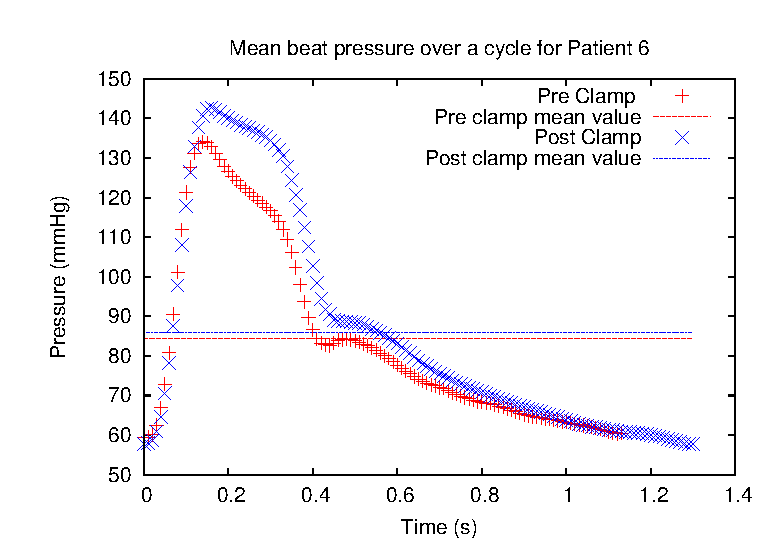
\includegraphics[scale=0.66]{Figures/Patient6.eps}
\end{minipage}
\begin{minipage}{0.48\textwidth}
\includegraphics[scale=0.66]{Figures/Patient7.eps}
\end{minipage}

\begin{minipage}{0.48\textwidth}
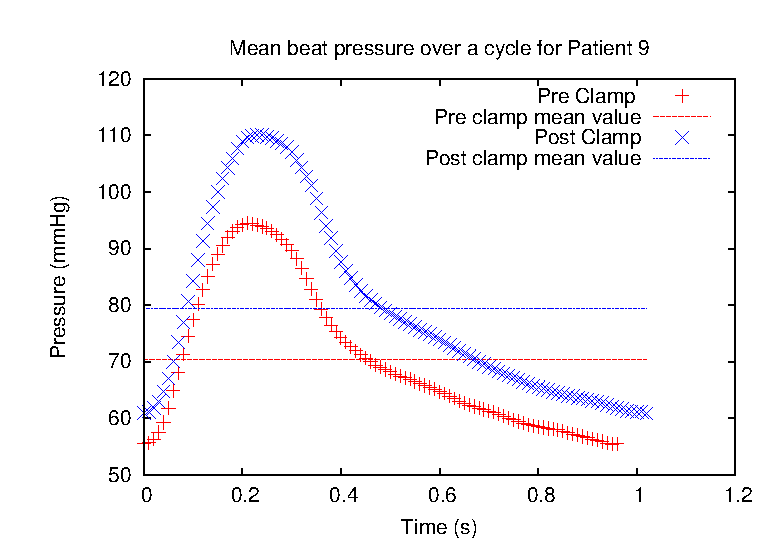
\includegraphics[scale=0.66]{Figures/Patient9.eps}
\end{minipage}
\begin{minipage}{0.48\textwidth}
\includegraphics[scale=0.66]{Figures/Patient14.eps}
\end{minipage}
\caption{Pressure wave signal for 4 patients undergoing aortic clamping during vascular surgery with their respective mean values. Red signals are pre clamp and blue signals are post clamp.}
\label{expe}
\end{figure}

The mean level of pressure tends to increase when clamping however the amounts in which it varies is highly patient-dependent. Nonetheless, the pressure wave morphology seems to be preserved by clamping, only the magnitude of the peak increases. It can also be seen that the heart time period tends to increase after clamping so the heart beat decreases. 

\section{1D numerical model}\label{numerical_sec}

First we introduce the model that describes blood flow and pressure wave propagation in the human arterial system. Blood flows in large arteries is described by a set of reduced 1D equations resulting from the integration of the reduced Navier-Stokes Prandtl equations of a cross-section of artery for an incompressible Newtonian fluid. It can be expressed in terms of the flow rate $Q$, the cross sectionnal area $A$ and the internal average pressure $P$ in the artery. 

\begin{equation}\label{1D_system}
\left\{\begin{array}{rl}
\displaystyle \frac{\partial A}{ \partial t } + \frac{\partial Q}{\partial x} = & 0 \\ 
\displaystyle \frac{\partial Q}{\partial t} + \frac{\partial }{\partial x} \left( \frac{Q^2}{A}\right) + \frac{A}{\rho} \frac{\partial p }{\partial x} =&  \displaystyle - C_f \frac{Q}{A} \\
\end{array} \right.
\end{equation}

where $\rho$ is the fluid density equal to 1 g/cm$^3$ for blood and $C_f$ the friction coefficient set to be equal to $22 \pi \nu$ \cite{Cf} with $\nu = $ 3.5 $10^{-2}$ cm$^2$/s, the kinematic viscosity of blood. The RHS of the second equation of system (\ref{1D_system}) is an approximation of the viscous drag. \\ 

Under the assumption that the arterial wall is thin ($h \ll R_0$), isotropic, homogeneous and incompressible, the pressure law links the internal pressure $p$ to the cross-sectionnal area $A$ through the following relationship: 

\begin{equation}\label{pressure_law}
p(x) - p_{ext} = K (\sqrt{A} - \sqrt{A_0}) +  K_{\nu} \frac{\partial A}{\partial t}
\end{equation}

where the parameter $K$ describes the elastic behavior of the wall and is of the following form:

\begin{equation}\label{elastic_part}
K = \frac{E }{1 - \nu^2}\frac{\sqrt{\pi} h}{A_0} 
\end{equation}

where $E$ is Young's modulus, $h$ the wall thickness, $\nu$ the Poisson coefficient and $A_0$ the initial cross section.  \\ 

The second term in the RHS of Eq. \ref{pressure_law} describes the viscoelastic behavior of the wall using a Kelvin-Voigt model \cite{viscoelastic}: 

\begin{equation}\label{viscoelastic_part}
K_{\nu} = \frac{\phi}{1 - \nu^2}\frac{\sqrt{\pi} h}{2 \sqrt{A_0} A }
\end{equation}

where $\phi$ is the wall viscoelastic coefficient. \\

Linearizing coefficient $K_{\nu}$ around $A_0$ allows to obtain the final set of equations:

\begin{equation}\label{system_final}
\left\{\begin{array}{rl}
\displaystyle \frac{\partial A}{ \partial t } + \frac{\partial Q}{\partial x} = & 0 \\ 
\displaystyle \frac{\partial Q}{\partial t} + \frac{\partial }{\partial x} \left( \frac{Q^2}{A}+ \frac{K}{3 \rho} A^{\frac{3}{2}}\right) =&  \displaystyle - C_f \frac{Q}{A} + C_{\nu} \frac{\partial ^2 Q}{\partial x^2}  \\
\end{array} \right.
\end{equation}

with $C_{\nu} =\displaystyle \frac{\phi}{1 - \nu^2}\frac{\sqrt{\pi} h}{2 \rho \sqrt{A_0} }$.

\section{Method}

The data acquisition takes place in the right radial artery sketched by the orange cross. The system of Eq. (\ref{system_final}) is solved in the 9-artery network (Fig. \ref{schema_pre} for pre clam and Fig. \ref{schema_post} for post clamp). Since, there is no data on the patient's heart function, we decided to model the heart as an input signal of the network. It is described in the next section.

\subsection{Input flow rate}

The inflow boundary condition is a flow rate thats mimics a heart pulse. The input flow rate is a half sine signal (see Fig. \ref{input_flow_rate}) described by two parameters: the amplitude $Q_0$ and the ejection time $T_{ej}$, which is a portion of heart beat $T$ fixed by the experimental data. We defined the following function: 

\begin{equation}\
f(t,\alpha) = \left\{ \begin{array}{ll}
\displaystyle \sin (\pi t/\alpha)  & ~ \text{ if }   ~ t < \alpha \\ 
\displaystyle 0    & ~ \text{ if }   ~ t > \alpha
\end{array} \right.
\end{equation}

The input flow rate is then defined as: 
\begin{equation}
Q_{input} (t) = Q_0 .  f(t/T - E(t/T), T_{ej})
\end{equation}

where $Q_0$ is the amplitude,  the function $E(t)$ is the integer-valued function, $T$ is the heart period and $T_{ej}$ is the ejection fraction. This function is represented in Fig. \ref{input_flow_rate}.

\begin{figure}[H]
\centering
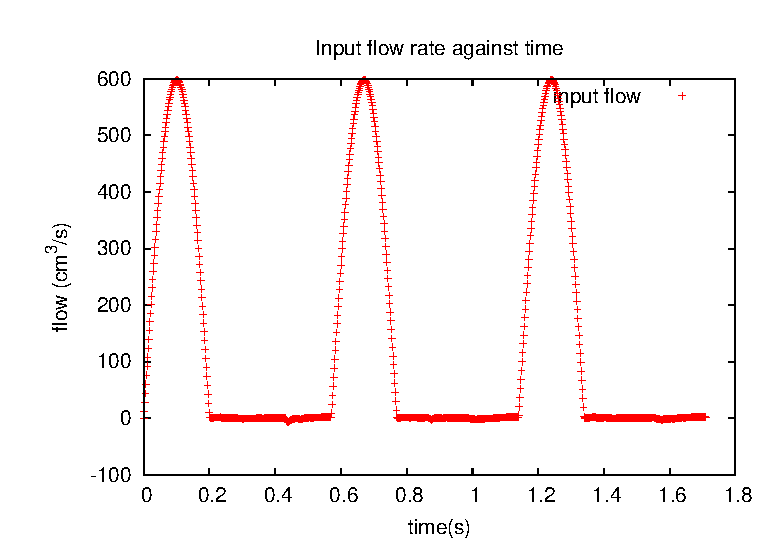
\includegraphics[scale=0.7]{Figures/input_flow.eps}
\caption{Input flow rate $Q$ as a function of time with amplitude $Q_0 =$ 600 cm$^3$/s and ejection time $T_{ej} = 35 \%$ of heart time period $T = 0.57$ s .}
\label{input_flow_rate}
\end{figure}

\subsection{Network}

The configuration of the sane 9-artery network is represented on Fig. \ref{schema_pre}. Reflection boundary conditions are applied to every terminal artery (sketched as blue squares in Fig. \ref{schema_pre} and \ref{schema_post}), taking values from the litterature and can be found in Table \ref{network}. The terminal vessel of the right arm (sketched with a yellow square) in which the pressure wave is measured requires a more detailed boundary condition so it is replaced by a three-element Windkessel model. The green circles separates each artery.  On Fig. \ref{schema_post}, the network is "cut" with a reflection coefficient of 1 that corresponds to a total obstruction of the vessel. Therefore the blood does not circulate in the lower part of the body and is reflected to only circulate in the upper part. We verify that at the end of the seventh artery the flow rate is equal to zero.  Table \ref{network} sums up the physiological data used for computations. 

\begin{figure}[H]
\centering
\includegraphics[scale=0.35]{Figures/Schema_pre.png}
\caption{Drawing of a 9-artery network in which the set of equations (\ref{system_final}) is being solved.}
\label{schema_pre}
\end{figure}

\begin{figure}[H]
\centering
\includegraphics[scale=0.35]{Figures/Schema_post.png}
\caption{Drawing of the 9-artery network after aortic clamping: the legs are replaced by a total reflection preventing any blood circulation in the legs.}
\label{schema_post}
\end{figure}

\begin{table}[H]
\begin{center}
\begin{tabular}{|c|c|c|c|c|c|c|}
\hline
N$^\circ$ & Name & L  (cm) & R (cm) & h (cm) & E (g.cm$^{-1}$.s$^{-2}$) & R$_t$ \\ 
\hline 
\hline
1 & Aorta arch A & 4.0 & 1.5 & 0.16 & 0.4e7 & ---\\
\hline 
2 & Right subclavian radial artery & 72.5 & 0.5 & 0.06 & 0.4e7 & ?  \\
\hline
3 & Aorta arch B & 2.0 & 1.3 & 0.12 & 0.4e7 &--- \\
\hline 
4 & Left carotid artery & 38.5 & 0.4 & 0.06 & 0.6e7 & 0.784 \\
\hline 
5 & Aorta arch C & 3.9 & 1.2 & 0.1 & 0.4e7 &---\\
\hline 
6 & Left subclavian radial artery & 69.1 & 0.4 & 0.06 & 0.4e7 & ?\\
\hline
7 & Aorta & 34.5  & 0.8 & 0.1 &0.4e7 & --- \\
\hline 
8 & Right femoral artery & 96.9 & 0.5 & 0.05 & 0.8e7 &0.724\\
\hline 
9 & Left femoral artery & 96.9  & 0.5 & 0.05 &0.8e7 &0.724 \\
\hline
\end{tabular}
\caption{Physiological data used in the 9-artery network model from \cite{bypass} and \cite{Saito9}. Question marks are the values that needs to be determined by the fitting of experimental data.}
\label{network}
\end{center}
\end{table}

\section{Results}

\subsection{Fitting of experimental data}

The experimental data is fitted by adjusting several parameters: the input amplitude of flow rate $Q_0$, the ejection time $T_{ej}$ (i.e. duration of systole) that can be seen of Fig. \ref{input_flow_rate}, the viscoelastic coefficient defined in Sec. \ref{numerical_sec}) and the Windkessel resistance $R_2$ and compliance $C$  (sketched on Fig \ref{schema_pre} and \ref{schema_post}). The first resistance $R_1$ is typically taken to be the impedance of the last vessel (here the right radial artery). The reflection coefficient corresponding to the Windkessel model will be applied for the left radial artery (artery number 6) with the following formula:

\begin{equation}\label{reflection_coeff}
R_t = \frac{R_2 - R_1 }{R_2 + R_1}
\end{equation} 

We look for a set of parameters $\mathbf{x} = (Q_0, T_{ej}, R_2, C, \nu_v)$ that minimizes a cost function defined as the difference between experimental data and numerical simulations. The tool used to quantify this minimization is the correlation coefficient R2 (function \texttt{sklearn.metrics.r2$\_$score}  from python3). \\

In the following sections, we show the parameter estimation for both pre clamp and post clamp cases for aortic clamping of patient 14. 

\subsubsection{Pre Clamp}

The four figures that follow show a rough idea of the parameter estimation. First figure (\ref{best_pre_clamp} top left) shows the best fit for the pre clamp pressure wave. Then the second figure (\ref{best_pre_clamp} top right) show the post clamp pressure wave but with the optimal parameters found for the pre clamp signal. It can be seen that these parameters do not fit the post clamp wave. The third figure (\ref{best_pre_clamp} bottom left) shows the post clamp pressure wave with the same parameters as the figures on top except for $Q_0$. This parameter increases the amplitude of the pressure wave. Then, it can be seen that the signal is still shifted towards the higher pressures. Therefore, we decide to decrease resistance with the value of $Q_0$ from Fig. \ref{best_pre_clamp} bottom left and plot it on  Fig. \ref{best_pre_clamp} bottom right. This last figure shows a roughly good match of simulated and experimental signals. 

\begin{figure}[H]
\begin{minipage}{0.48 \textwidth}
\centering
\includegraphics[scale=0.52]{Figures/Best_pre_clamp.eps}
\end{minipage}
\begin{minipage}{0.48 \textwidth}
\includegraphics[scale=0.52]{Figures/postclamp_pre.eps}
\end{minipage}

\begin{minipage}{0.48 \textwidth}
\centering
\includegraphics[scale=0.52]{Figures/postclamp_QR.eps}
\end{minipage}
\begin{minipage}{0.48 \textwidth}
\includegraphics[scale=0.52]{Figures/postclamp_Q.eps}
\end{minipage}

\caption{Left: Optimal set of parameters for comparison between experimental and numerical pre clamp pressure waves in the right radial artery. The correlation coefficient $R^2 $ is equal to 0.65. Black line represents the experimental measurements, red is the simulated pressure wave. Optimal values are: $Q_0 = 300 $ cm$^3$/s, $T_{ej}= $ 50 $\%$ of $T = 0.57 $ s, $R_1$ is taken to be the impedance of the last vessel and is equal to 720 g.cm$^{-4}$.s$^{-1}$, $R_2 = 5000 $ g.cm$^{-4}$.s$^{-1}$, and C = $10^{-6}$ g$^{-1}$.cm$^{4}$.s$^{2}$ and $\nu_v = 31 ~ 10^4$. Top right: Post clamp pressure wave with optimal parameters of pre clamp. Bottom left: Post clamp pressure wave changing $Q_0$. Bottom right: Post clamp pressure wave changing $R_2$. }
\label{best_pre_clamp}
\end{figure}

\begin{table}[H]
\begin{center}
\begin{tabular}{|c|c|c|}
\hline
 & Pre Clamp & Post Clamp  \\
\hline 
R2 & 0.65 & 0.75 \\
\hline 
\end{tabular}
\caption{Correlation coefficient from Fig. \ref{best_pre_clamp}. Pre clamp value corresponds to top left figure and post clamp corresponds to bottom right figure.}
\label{final_results}
\end{center}
\end{table}
\begin{figure}[H]

\centering
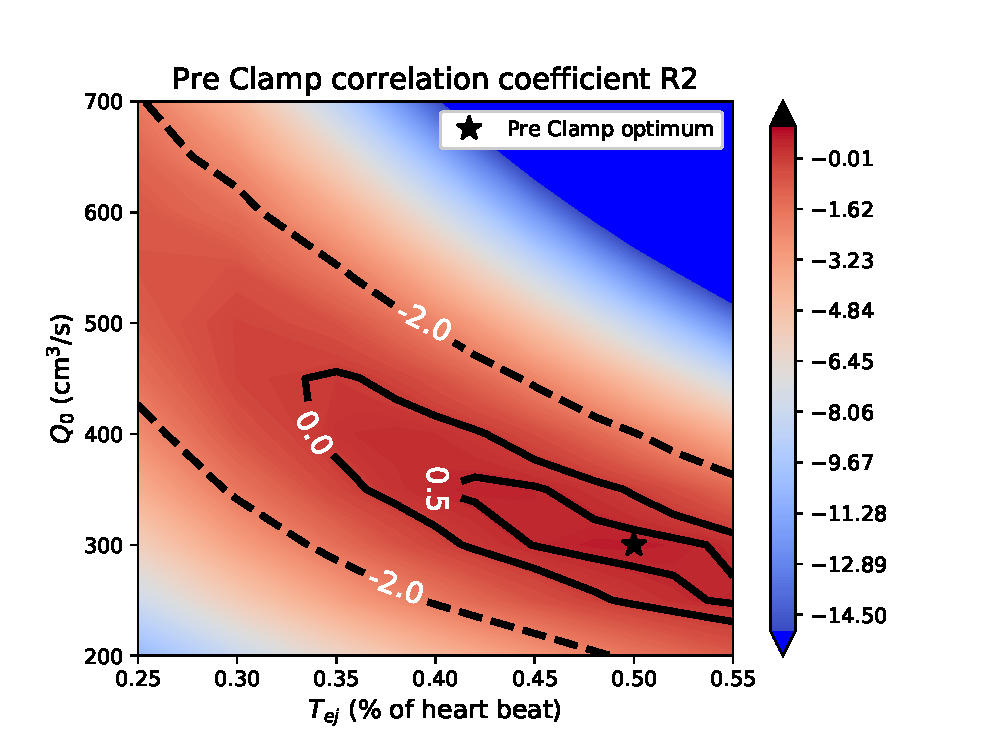
\includegraphics[scale=0.7]{Figures/preclamp_phase_diagram_QTej.eps}
\caption{Phase diagram showing the correlation coefficient as a function of $Q_0$ and $T_{ej}$. The black star represents the optimal combination of these two parameters in the pre clamp situation ($R^2 = $0.65).}
\label{PD_preclamp}
\end{figure}

\begin{figure}[H]
\centering
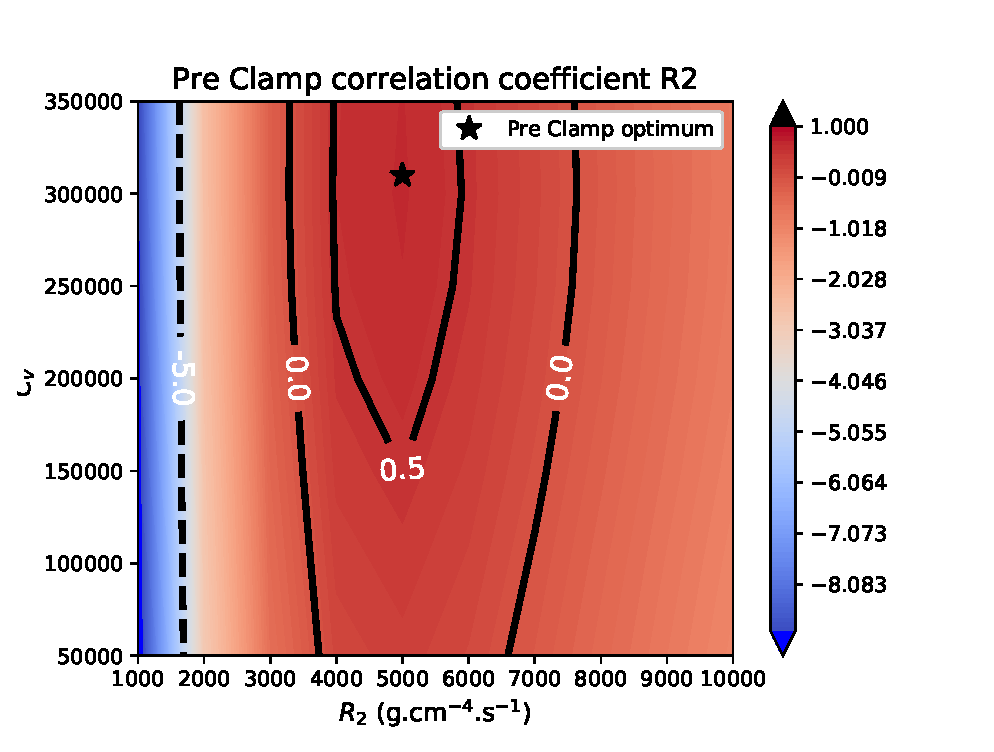
\includegraphics[scale=0.7]{Figures/preclamp_phase_diagram_nuv.eps}
\caption{Phase diagram showing the correlation coefficient as a function of the viscoelastic coefficient $\nu_v$ and the resistance $R_2$. The black star represents the optimal combination of these two parameters in the pre clamp situation ($R^2 = $0.65). }
\label{PD_preclamp_nu}
\end{figure}

\subsubsection{Post Clamp}

In the following, we try to find the best fit for the post clamp situation regardless of the values found for the pre clamp situation. 

\begin{figure}[H]
\centering
\includegraphics[scale=0.7]{Figures/postclamp_phase_diagram.eps}
\caption{Phase diagram showing the correlation coefficient as a function of $Q_0$ and $T_{ej}$. The black star represents the optimal combination of these two parameters in the post clamp situation ($R^2 = $0.97). }
\label{PD_postclamp}
\end{figure}

\begin{figure}[H]
\centering
\includegraphics[scale=0.7]{Figures/postclamp.eps}
\caption{Optimal set of parameters for comparison between experimental and numerical post clamp pressure waves in the right radial artery. The correlation coefficient $R^2 $ is equal to 0.97 in the figure. Black line represents the experimental measurements, red is the simulated pressure wave. Optimal values are : $Q_0 = 600 $ cm$^3$/s, $T_{ej}= $ 36 $\%$ of $T = 0.62 $ s, $R_1$ is taken to be the impedance of the last vessel and is equal to 720 g.cm$^{-4}$.s$^{-1}$, $R_2 = 1750 $ g.cm$^{-4}$.s$^{-1}$, and C = $10^{-6}$ g$^{-1}$.cm$^{4}$.s$^{2}$ and $\nu_v = 5 ~ 10^4$.}
\label{post_clamp}
\end{figure}

\subsubsection{Comparison }

We define the percentage of change of variable $x$ as : 

\begin{equation}
\% = \frac{\Delta x}{x} 
\end{equation}

where $\Delta x$ is $|x_{pre} - x_{post}|$. 

\begin{table}[H]
\begin{center}
\begin{tabular}{|c|c|c|c|}
\hline
Parameters & Pre Clamp & Post Clamp & $\% $ of change \\
\hline 
$Q_0$ (cm$^3$/s)  & & 600 & \\ 
\hline 
$T_{ej} $ ($\%$) & & 36 & \\
\hline 
$R_2$  (g.cm$^{-4}$.s$^{-1}$) &  & 1750 & \\ 
\hline 
$C$ (g$^{-1}$.cm$^{4}$.s$^{2}$) &  & $10^{-6}$ & 0 \\
\hline
$\nu_v$ & & 5 10$^4$ & \\  
\hline
\hline 
$R^2$ coefficient & 0.65 & 0.97 & ---\\ 
\hline
\end{tabular}
\caption{Parameters that maximise the correlation coefficient R2 that links the experimental measurements of pressure in the right radial artery and numerical simulation. }
\label{final_results}
\end{center}
\end{table}

\section{Conclusions}

\nocite{*}
\bibliographystyle{plain}
\bibliography{biblio}



\end{document}
